\documentclass{standalone}
\usepackage{tikz}

\begin{document}

\tikzstyle{lightedge}=[blue]
\tikzstyle{mainedge}=[red,very thick]
\tikzstyle{inputBit}=[rectangle,fill=red, text=white]
\tikzstyle{outputBit}=[rectangle,fill=blue, text=white]
\tikzstyle{pointer}=[orange,->,dashed]

\newcounter{ctra}
\newcommand{\trellisEdges}[2]{%
    \setcounter{ctra}{#2}
    \pgfmathtruncatemacro{\xplusone}{#1 + 1}
    \ifodd\value{ctra}
        \draw[mainedge] (s#1#2) -- (s\xplusone2);
    \else
        \draw[mainedge] (s#1#2) -- (s\xplusone0);
    \fi%
    \ifodd\value{ctra}
        \draw[lightedge] (s#1#2) -- (s\xplusone3);
    \else
        \draw[lightedge] (s#1#2) -- (s\xplusone1);
    \fi%
}

% #1=x; #2=y; #3=In; #4=Out
\newcommand{\trellisInOut}[4]{
    \node[inputBit] (in#1) at (#1+0.5,5) {#3};
    \node[outputBit] (out#1) at (#1+0.5,6) {#4};
    \draw[pointer] (in#1) -- (#1+0.5,#2);
}

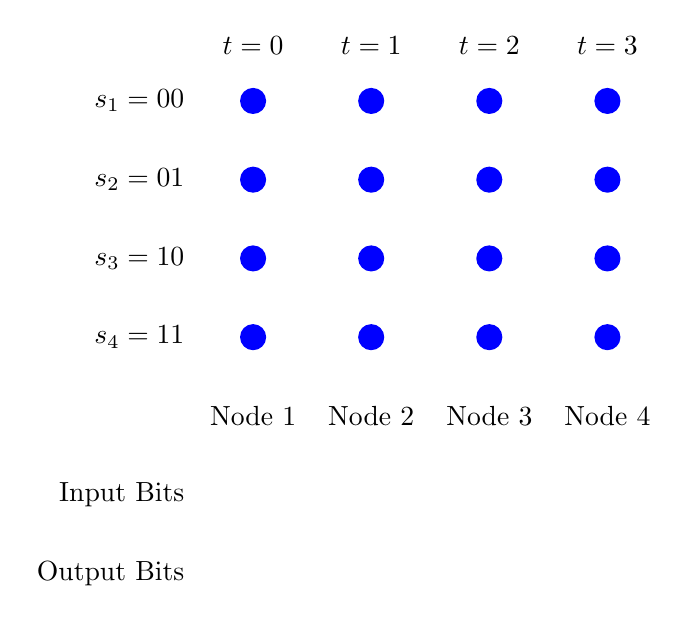
\begin{tikzpicture}[x=1.5cm, y=-1cm]
    \node at (-0.5,0) [left] {$s_1=00$};
    \node at (-0.5,1) [left] {$s_2=01$};
    \node at (-0.5,2) [left] {$s_3=10$};
    \node at (-0.5,3) [left] {$s_4=11$};

    % Nodes
    \foreach \x in {0,...,3} {
        \node at (\x,-.7) {$t=\x$};
        \foreach \y in {0,...,3} {
            \node (s\x\y) at (\x,\y) [circle,fill=blue] {};
        }
        \node at (\x,4) {
            \pgfmathparse{\x+1}
            Node \pgfmathprintnumber[fixed,fixed zerofill,precision=0]{\pgfmathresult}
        };
    }

    % Edges
    \trellisEdges{0}{0}
    \trellisEdges{1}{0}
    \trellisEdges{1}{1}
    \trellisEdges{2}{0}
    \trellisEdges{2}{1}
    \trellisEdges{2}{2}
    \trellisEdges{2}{3}

    % Inputs and Outputs
    \node at (-0.5,5) [left] {Input Bits};
    \node at (-0.5,6) [left] {Output Bits};

    \trellisInOut{0}{0.5}{1}{11}
    \trellisInOut{1}{2.0}{1}{01}
    \trellisInOut{2}{2.5}{0}{01}
\end{tikzpicture}

\end{document}